\documentclass[tikz,border=4pt]{standalone}
\usepackage{ctex}
\usepackage{amsmath}
\usepackage{pgfplots}
\pgfplotsset{compat=1.18}

% p10-07a: 含参二次函数——参数影响对称轴位置
% y=x^2-2bx+1，对称轴x=b，不同b值对应不同对称轴
\begin{document}
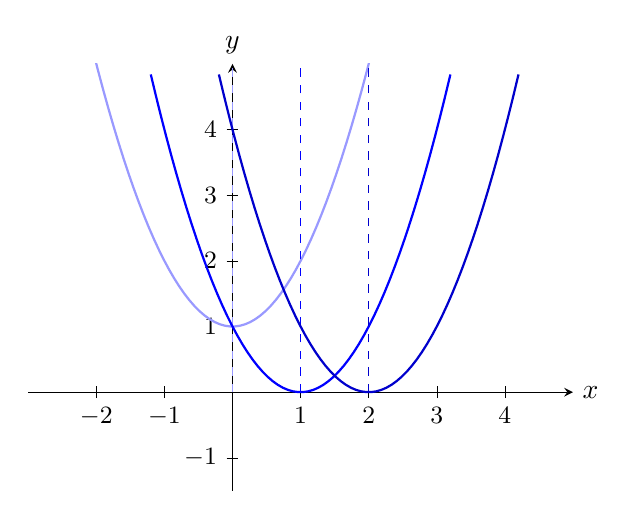
\begin{tikzpicture}
\begin{axis}[
  width=8.5cm, height=7cm,
  axis lines=center,
  xlabel={$x$}, ylabel={$y$},
  every axis x label/.style={at={(axis cs:5.0,0)}, anchor=west},
  every axis y label/.style={at={(axis cs:0,5.0)}, anchor=south},
  xmin=-3.0, xmax=5.0,
  ymin=-1.5, ymax=5.0,
  xtick={-2,-1,1,2,3,4},
  ytick={-1,1,2,3,4},
  tick style={color=black},
  ticklabel style={font=\small},
  clip=true,
]
  % b=0: y=x^2+1，对称轴x=0
  \addplot[blue!40, thick, domain=-2.2:2.2, samples=60] {x^2+1};
  \draw[blue!40, dashed] (axis cs:0,0) -- (axis cs:0,5.0);
  \node[above, blue!40, font=\tiny] at (axis cs:0,5.0) {$b=0$};

  % b=1: y=x^2-2x+1=(x-1)^2，对称轴x=1
  \addplot[blue, thick, domain=-1.2:3.2, samples=60] {(x-1)^2};
  \draw[blue, dashed] (axis cs:1,0) -- (axis cs:1,5.0);
  \node[above, blue, font=\tiny] at (axis cs:1,5.0) {$b=1$};

  % b=2: y=x^2-4x+4=(x-2)^2，对称轴x=2
  \addplot[blue!80!black, thick, domain=-0.2:4.2, samples=60] {(x-2)^2};
  \draw[blue!80!black, dashed] (axis cs:2,0) -- (axis cs:2,5.0);
  \node[above, blue!80!black, font=\tiny] at (axis cs:2,5.0) {$b=2$};
\end{axis}
\end{tikzpicture}
\end{document}
